\documentclass[12pt,twoside]{article}
\usepackage[noae]{Sweave}
\usepackage{caxetexFree}
\usepackage{lipsum}
\usepackage{titlesec}
\usepackage{bm}
\titleformat{\paragraph}[runin]{\normalfont\normalsize\textsb}{\theparagraph}{1em}{}
\newcommand{\myTitle}{Judicial behaviour, part 2}
\title{\myTitle}
\author{Chris Hanretty}
\date{6th May 2016}
\newcommand{\chaptermark}

%% From https://github.com/minrk/ipython/commit/325e76d80861d5cec65b08396c39c6316cde0912

    % commands and environments needed by pandoc snippets
    % extracted from the output of `pandoc -s`
    
    \DefineShortVerb[commandchars=\\\{\}]{\|}
    \DefineVerbatimEnvironment{Highlighting}{Verbatim}{commandchars=\\\{\}}
    % Add ',fontsize=\small' for more characters per line
    \newenvironment{Shaded}{}{}
    \newcommand{\KeywordTok}[1]{\textcolor[rgb]{0.00,0.44,0.13}{\textbf{{#1}}}}
    \newcommand{\DataTypeTok}[1]{\textcolor[rgb]{0.56,0.13,0.00}{{#1}}}
    \newcommand{\DecValTok}[1]{\textcolor[rgb]{0.25,0.63,0.44}{{#1}}}
    \newcommand{\BaseNTok}[1]{\textcolor[rgb]{0.25,0.63,0.44}{{#1}}}
    \newcommand{\FloatTok}[1]{\textcolor[rgb]{0.25,0.63,0.44}{{#1}}}
    \newcommand{\CharTok}[1]{\textcolor[rgb]{0.25,0.44,0.63}{{#1}}}
    \newcommand{\StringTok}[1]{\textcolor[rgb]{0.25,0.44,0.63}{{#1}}}
    \newcommand{\CommentTok}[1]{\textcolor[rgb]{0.38,0.63,0.69}{\textit{{#1}}}}
    \newcommand{\OtherTok}[1]{\textcolor[rgb]{0.00,0.44,0.13}{{#1}}}
    \newcommand{\AlertTok}[1]{\textcolor[rgb]{1.00,0.00,0.00}{\textbf{{#1}}}}
    \newcommand{\FunctionTok}[1]{\textcolor[rgb]{0.02,0.16,0.49}{{#1}}}
    \newcommand{\RegionMarkerTok}[1]{{#1}}
    \newcommand{\ErrorTok}[1]{\textcolor[rgb]{1.00,0.00,0.00}{\textbf{{#1}}}}
    \newcommand{\NormalTok}[1]{{#1}}
\providecommand{\tightlist}{%
  \setlength{\itemsep}{0pt}\setlength{\parskip}{0pt}}    
\pagestyle{fancy}
\renewcommand{\chaptermark}[1]{\markboth{#1}{}}
\fancyhead{} % clear all header fields
\fancyhead[CE]{\rightmark}
\fancyhead[CO]{\leftmark}
\fancyfoot{} % clear all footer fields
\fancyfootoffset[RO]{-0.25in}
\fancyfootoffset[LE]{-0.25in}
\fancyfootoffset[RE]{-0.25in}
\fancyfootoffset[LO]{-0.25in}
\fancyfoot[RO]{\thepage}
\fancyfoot[LE]{\thepage}
\fancyfoot[RE]{\texttt{\jobname{}.tex}, \textsf{revised \today}}
\fancyfoot[LO]{\texttt{\jobname{}.tex}, \textsf{revised \today}}

\renewcommand{\headrulewidth}{0pt}  %1.4

\setlength{\footskip}{33pt}

% Create headerless version for "plain" pages, 
% e.g., page 1 of a paper
\fancypagestyle{plain}{%
\fancyhf{} % clear all header and footer fields
\fancyfootoffset[RO]{-0.25in}
\fancyfootoffset[LE]{-0.25in}
\fancyfootoffset[RE]{-0.25in}
\fancyfootoffset[LO]{-0.25in}
\fancyfoot[RO]{\thepage}
\fancyfoot[LE]{\thepage}
\fancyfoot[RE]{\texttt{\jobname{}.tex}, \textsf{revised \today}}
\fancyfoot[LO]{\texttt{\jobname{}.tex}, \textsf{revised \today}}
\renewcommand{\headrulewidth}{0pt}
\renewcommand{\footrulewidth}{0pt}}

 \renewcommand{\leftmark}{\textsc{\caps{chris hanretty}}~~\(\cdot\)~~\emph{\textsb{%
\myTitle{}%
}}}
 \renewcommand{\rightmark}{\textsc{\caps{chris hanretty}}~~\(\cdot\)~~\emph{\textsb{%
\myTitle{}%
}}}



\begin{document}
\maketitle

\section{Ideal point analysis}\label{ideal-point-analysis}

\subsection{The key idea}\label{the-key-idea}

\begin{itemize}
\tightlist
\item
  Before, we looked at variation across cases
\item
  We needed random assignment to exclude differences in outcome
  resulting from differences in cases
\item
  There is also variation \emph{within} cases
\item
  That is, judges can dissent, and this can permit inferences about
  their ideology
\end{itemize}

\subsection{Not universally
applicable}\label{not-universally-applicable}

\begin{itemize}
\tightlist
\item
  Not every court allows (signed) dissenting opinions
\item
  In such cases, these models can't apply
\item
  But see Malecki, M. (2012). Do ECJ judges all speak with the same
  voice? Evidence of divergent preferences from the judgments of
  chambers. \emph{Journal of European Public Policy}, 19(1), 59-75.
\end{itemize}

\subsection{Start simple}\label{start-simple}

\begin{itemize}
\tightlist
\item
  I'll be using the most common database of judicial behaviour,the
  Spaeth database
\item
  You can find it at \url{scdb.wustl.edu}
\item
  The database is in a \emph{long} format (one row = one judge/case)
\item
  You will need to convert it to a \emph{wide} format
\end{itemize}

\subsection{The first few lines of
Spaeth}\label{the-first-few-lines-of-spaeth}

\tiny

\begin{longtable}[c]{@{}ccccccc@{}}
\caption{Table continues below}\tabularnewline
\toprule
\begin{minipage}[b]{0.10\columnwidth}\centering\strut
~
\strut\end{minipage} &
\begin{minipage}[b]{0.10\columnwidth}\centering\strut
caseId
\strut\end{minipage} &
\begin{minipage}[b]{0.13\columnwidth}\centering\strut
AMKennedy
\strut\end{minipage} &
\begin{minipage}[b]{0.11\columnwidth}\centering\strut
AScalia
\strut\end{minipage} &
\begin{minipage}[b]{0.11\columnwidth}\centering\strut
CThomas
\strut\end{minipage} &
\begin{minipage}[b]{0.10\columnwidth}\centering\strut
EKagan
\strut\end{minipage} &
\begin{minipage}[b]{0.12\columnwidth}\centering\strut
JGRoberts
\strut\end{minipage}\tabularnewline
\midrule
\endfirsthead
\toprule
\begin{minipage}[b]{0.10\columnwidth}\centering\strut
~
\strut\end{minipage} &
\begin{minipage}[b]{0.10\columnwidth}\centering\strut
caseId
\strut\end{minipage} &
\begin{minipage}[b]{0.13\columnwidth}\centering\strut
AMKennedy
\strut\end{minipage} &
\begin{minipage}[b]{0.11\columnwidth}\centering\strut
AScalia
\strut\end{minipage} &
\begin{minipage}[b]{0.11\columnwidth}\centering\strut
CThomas
\strut\end{minipage} &
\begin{minipage}[b]{0.10\columnwidth}\centering\strut
EKagan
\strut\end{minipage} &
\begin{minipage}[b]{0.12\columnwidth}\centering\strut
JGRoberts
\strut\end{minipage}\tabularnewline
\midrule
\endhead
\begin{minipage}[t]{0.10\columnwidth}\centering\strut
\textbf{7}
\strut\end{minipage} &
\begin{minipage}[t]{0.10\columnwidth}\centering\strut
2010-007
\strut\end{minipage} &
\begin{minipage}[t]{0.13\columnwidth}\centering\strut
1
\strut\end{minipage} &
\begin{minipage}[t]{0.11\columnwidth}\centering\strut
0
\strut\end{minipage} &
\begin{minipage}[t]{0.11\columnwidth}\centering\strut
1
\strut\end{minipage} &
\begin{minipage}[t]{0.10\columnwidth}\centering\strut
1
\strut\end{minipage} &
\begin{minipage}[t]{0.12\columnwidth}\centering\strut
1
\strut\end{minipage}\tabularnewline
\begin{minipage}[t]{0.10\columnwidth}\centering\strut
\textbf{15}
\strut\end{minipage} &
\begin{minipage}[t]{0.10\columnwidth}\centering\strut
2010-015
\strut\end{minipage} &
\begin{minipage}[t]{0.13\columnwidth}\centering\strut
1
\strut\end{minipage} &
\begin{minipage}[t]{0.11\columnwidth}\centering\strut
1
\strut\end{minipage} &
\begin{minipage}[t]{0.11\columnwidth}\centering\strut
1
\strut\end{minipage} &
\begin{minipage}[t]{0.10\columnwidth}\centering\strut
1
\strut\end{minipage} &
\begin{minipage}[t]{0.12\columnwidth}\centering\strut
1
\strut\end{minipage}\tabularnewline
\begin{minipage}[t]{0.10\columnwidth}\centering\strut
\textbf{16}
\strut\end{minipage} &
\begin{minipage}[t]{0.10\columnwidth}\centering\strut
2010-016
\strut\end{minipage} &
\begin{minipage}[t]{0.13\columnwidth}\centering\strut
1
\strut\end{minipage} &
\begin{minipage}[t]{0.11\columnwidth}\centering\strut
1
\strut\end{minipage} &
\begin{minipage}[t]{0.11\columnwidth}\centering\strut
0
\strut\end{minipage} &
\begin{minipage}[t]{0.10\columnwidth}\centering\strut
1
\strut\end{minipage} &
\begin{minipage}[t]{0.12\columnwidth}\centering\strut
1
\strut\end{minipage}\tabularnewline
\begin{minipage}[t]{0.10\columnwidth}\centering\strut
\textbf{19}
\strut\end{minipage} &
\begin{minipage}[t]{0.10\columnwidth}\centering\strut
2010-019
\strut\end{minipage} &
\begin{minipage}[t]{0.13\columnwidth}\centering\strut
1
\strut\end{minipage} &
\begin{minipage}[t]{0.11\columnwidth}\centering\strut
0
\strut\end{minipage} &
\begin{minipage}[t]{0.11\columnwidth}\centering\strut
1
\strut\end{minipage} &
\begin{minipage}[t]{0.10\columnwidth}\centering\strut
1
\strut\end{minipage} &
\begin{minipage}[t]{0.12\columnwidth}\centering\strut
1
\strut\end{minipage}\tabularnewline
\bottomrule
\end{longtable}

\begin{longtable}[c]{@{}ccccc@{}}
\toprule
\begin{minipage}[b]{0.11\columnwidth}\centering\strut
~
\strut\end{minipage} &
\begin{minipage}[b]{0.16\columnwidth}\centering\strut
RBGinsburg
\strut\end{minipage} &
\begin{minipage}[b]{0.12\columnwidth}\centering\strut
SAAlito
\strut\end{minipage} &
\begin{minipage}[b]{0.13\columnwidth}\centering\strut
SGBreyer
\strut\end{minipage} &
\begin{minipage}[b]{0.14\columnwidth}\centering\strut
SSotomayor
\strut\end{minipage}\tabularnewline
\midrule
\endhead
\begin{minipage}[t]{0.11\columnwidth}\centering\strut
\textbf{7}
\strut\end{minipage} &
\begin{minipage}[t]{0.16\columnwidth}\centering\strut
1
\strut\end{minipage} &
\begin{minipage}[t]{0.12\columnwidth}\centering\strut
1
\strut\end{minipage} &
\begin{minipage}[t]{0.13\columnwidth}\centering\strut
1
\strut\end{minipage} &
\begin{minipage}[t]{0.14\columnwidth}\centering\strut
1
\strut\end{minipage}\tabularnewline
\begin{minipage}[t]{0.11\columnwidth}\centering\strut
\textbf{15}
\strut\end{minipage} &
\begin{minipage}[t]{0.16\columnwidth}\centering\strut
0
\strut\end{minipage} &
\begin{minipage}[t]{0.12\columnwidth}\centering\strut
1
\strut\end{minipage} &
\begin{minipage}[t]{0.13\columnwidth}\centering\strut
1
\strut\end{minipage} &
\begin{minipage}[t]{0.14\columnwidth}\centering\strut
0
\strut\end{minipage}\tabularnewline
\begin{minipage}[t]{0.11\columnwidth}\centering\strut
\textbf{16}
\strut\end{minipage} &
\begin{minipage}[t]{0.16\columnwidth}\centering\strut
0
\strut\end{minipage} &
\begin{minipage}[t]{0.12\columnwidth}\centering\strut
1
\strut\end{minipage} &
\begin{minipage}[t]{0.13\columnwidth}\centering\strut
1
\strut\end{minipage} &
\begin{minipage}[t]{0.14\columnwidth}\centering\strut
1
\strut\end{minipage}\tabularnewline
\begin{minipage}[t]{0.11\columnwidth}\centering\strut
\textbf{19}
\strut\end{minipage} &
\begin{minipage}[t]{0.16\columnwidth}\centering\strut
0
\strut\end{minipage} &
\begin{minipage}[t]{0.12\columnwidth}\centering\strut
1
\strut\end{minipage} &
\begin{minipage}[t]{0.13\columnwidth}\centering\strut
1
\strut\end{minipage} &
\begin{minipage}[t]{0.14\columnwidth}\centering\strut
1
\strut\end{minipage}\tabularnewline
\bottomrule
\end{longtable}

By convention, `1' = a vote with the majority.

\subsection{Simple measures}\label{simple-measures}

\begin{itemize}
\tightlist
\item
  The average rate at which judges agree is 75 percent
\item
  The lowest rate of agreement between two judges is 59 percent
\item
  This is between RBGinsburg and CThomas.
\item
  Is this rate significantly lower than average?
\end{itemize}

\subsection{Simple tests for simple
measures}\label{simple-tests-for-simple-measures}

\small

\begin{Shaded}
\begin{Highlighting}[]
\NormalTok{times.judges.agreed <-}\StringTok{ }\DecValTok{228}
\NormalTok{times.judges.sat.together <-}\StringTok{ }\DecValTok{387}
\KeywordTok{binom.test}\NormalTok{(times.judges.agreed,}
           \NormalTok{times.judges.sat.together,}
           \DataTypeTok{p =} \FloatTok{0.75}\NormalTok{)}
\end{Highlighting}
\end{Shaded}

\begin{verbatim}
## 
##  Exact binomial test
## 
## data:  times.judges.agreed and times.judges.sat.together
## number of successes = 228, number of trials = 387, p-value =
## 5.261e-12
## alternative hypothesis: true probability of success is not equal to 0.75
## 95 percent confidence interval:
##  0.5383110 0.6386093
## sample estimates:
## probability of success 
##              0.5891473
\end{verbatim}

\subsection{A UK counterexample}\label{a-uk-counterexample}

\begin{itemize}
\tightlist
\item
  Dissent is less common on the UK Supreme Court\ldots{}
\item
  but judges are often seen as `small-c conservative' or not
\item
  one interesting judge pairing: Lady Hale and Lord Sumption
\item
  Do they also agree at below average rates?
\end{itemize}

\subsection{Hale/Sumption}\label{halesumption}

\begin{Shaded}
\begin{Highlighting}[]
\NormalTok{times.judges.agreed <-}\StringTok{ }\DecValTok{21}
\NormalTok{times.judges.sat.together <-}\StringTok{ }\DecValTok{26}
\KeywordTok{binom.test}\NormalTok{(times.judges.agreed,}
           \NormalTok{times.judges.sat.together,}
           \DataTypeTok{p =} \FloatTok{0.84}\NormalTok{)}
\end{Highlighting}
\end{Shaded}

\begin{verbatim}
## 
##  Exact binomial test
## 
## data:  times.judges.agreed and times.judges.sat.together
## number of successes = 21, number of trials = 26, p-value = 0.5954
## alternative hypothesis: true probability of success is not equal to 0.84
## 95 percent confidence interval:
##  0.6064945 0.9344519
## sample estimates:
## probability of success 
##              0.8076923
\end{verbatim}

Lesson of the tale? Before you get advanced, get simple.

\subsection{Why can't we proceed in this
way?}\label{why-cant-we-proceed-in-this-way}

\begin{itemize}
\tightlist
\item
  We could calculate pairwise rates of agreement
\item
  We could arrange judges by similarity
\item
  But the number of comparisons grows exponentially:

  \begin{itemize}
  \tightlist
  \item
    Three-judge court: 3 comparisons
  \item
    Five-judge court: 10 comparisons
  \item
    Nine-judge court: 36 comparisons
  \end{itemize}
\item
  We need something that makes differences between judges stand out
\end{itemize}

\subsection{Notation}\label{notation}

\begin{itemize}
\tightlist
\item
  I'll use \(j\) to refer to judges 1 through \(J\)
\item
  I'll use \(i\) to refer to cases 1 through \(I\)
\item
  Each judge is assumed to have an ideal point, \(\theta_j\) (theta-j)
\item
  That's a point in a (one-dimensional) space
\item
  Often, smaller numbers = more left-wing
\end{itemize}

\subsection{More notation}\label{more-notation}

\begin{itemize}
\tightlist
\item
  Each case will have a \emph{location} or a \emph{cutpoint}
\item
  I'll denote this using \(\alpha_i\)
\item
  This is defined relative to judges' votes
\item
  The cutpoint is supposed to divide judges who vote one way from judges
  who vote another way
\end{itemize}

\subsection{The outcome}\label{the-outcome}

\begin{itemize}
\tightlist
\item
  Here, we'll be trying to explain the judge's vote
\item
  I'll use \(y_{ij}\) to refer to that
\item
  By convention, \(y_{ij}=1\) when the judge votes with the majority
\item
  For the moment, let's assume the majority is always conservative
\end{itemize}

\subsection{The relationship, visually}\label{the-relationship-visually}

\begin{figure}[htbp]
\centering
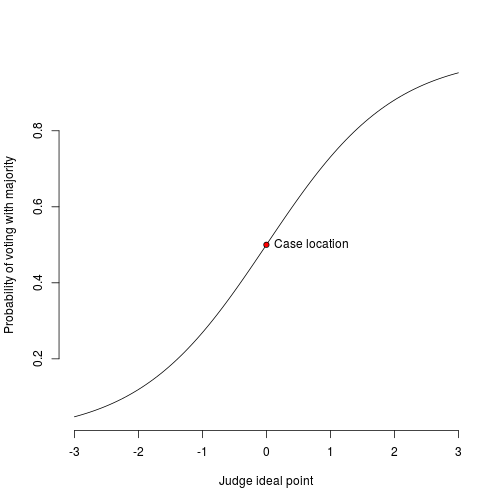
\includegraphics{figure/irtfig1-1.png}
\caption{Probability of voting with majority}
\end{figure}

\subsection{The relationship, in
equations}\label{the-relationship-in-equations}

\[
p = \frac{1}{1 + e^{-a + bx}}
\]

I'm going to replace two of the letters in that equation by the
specialised terms we used before, and scrub out the b.

\[
p = \frac{1}{1 + e^{-\alpha_i + \theta_j}}
\]

Alternately,

\[
p = \frac{1}{1 + e^{\theta_j-\alpha_i}}
\]

\subsection{The problem}\label{the-problem}

\begin{itemize}
\tightlist
\item
  Not all cases can be guaranteed to be related to ideology in the same
  way
\item
  The relationship might be weaker (the slope of the curve might be
  flatter)
\item
  The relationship might go the other way
\item
  To cope with this, we'll introduce a \emph{case discrimination
  parameter}, \(\beta\)
\end{itemize}

\subsection{Varying discrimination
parameters}\label{varying-discrimination-parameters}

\begin{figure}[htbp]
\centering
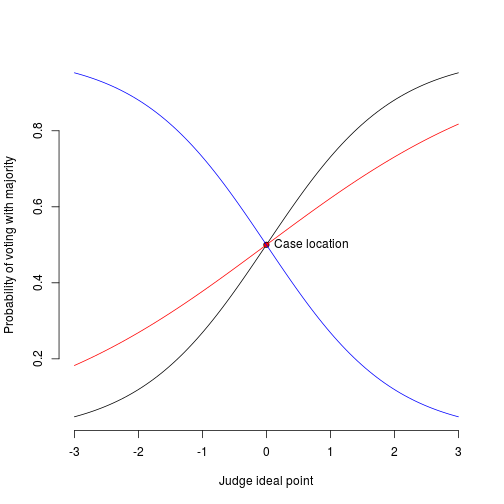
\includegraphics{figure/casediscrim-1.png}
\caption{Varying discrimination parameters}
\end{figure}

\subsection{The task}\label{the-task}

\begin{quote}
``Dear computer, Please find values of \(\alpha\), \(\beta\), and
\(\theta\) that best make sense of the pattern of votes we see. Yours,
Chris''
\end{quote}

\begin{itemize}
\tightlist
\item
  Estimation is through Markov Chain Monte Carlo.
\item
  Take some starting estimates (`guesses') of the values
\item
  Jump around a bit, and if the fit got better, keep those values
\item
  Repeat until you're fairly sure the values you have don't depend on
  your starting values
\end{itemize}

\subsection{Making it easier}\label{making-it-easier}

\begin{itemize}
\tightlist
\item
  We can get rid of all unanimous cases
\item
  These cases contribute nothing to our knowledge of the parameters
\item
  The case location parameter could be either far to the left, or far to
  the right
\item
  It's impossible to tell
\end{itemize}

\subsection{One problem}\label{one-problem}

\begin{itemize}
\tightlist
\item
  As it stands, our model is not \emph{identified}
\item
  (That is, we cannot uniquely identify good values)
\item
  Multiply everything by minus 1, flipping it around? No change
\item
  Scale everything by dividing it by a constant? No change
\end{itemize}

\subsection{Identification
constraints}\label{identification-constraints}

\begin{itemize}
\tightlist
\item
  Common to fix two judges as `anchor' judges
\item
  set, e.g., a left-wing judge to -1, a right-wing judge to +1
\item
  Sets both scale and direction
\end{itemize}

\subsection{Implementation}\label{implementation}

\begin{itemize}
\tightlist
\item
  Two common packages:

  \begin{itemize}
  \tightlist
  \item
    \texttt{MCMCpack}, and its function \texttt{MCMCirt1d}
  \item
    \texttt{pscl} and its function \texttt{ideal}
  \end{itemize}
\item
  I would probably recommend \texttt{pscl}
\item
  Both packages require data with judges down the rows
\end{itemize}

\subsection{Prepping the data}\label{prepping-the-data}

\begin{Shaded}
\begin{Highlighting}[]
\NormalTok{### Get the third column to the last column}
\NormalTok{vote.mat <-}\StringTok{ }\NormalTok{scdb.c[,}\DecValTok{3}\NormalTok{:}\KeywordTok{ncol}\NormalTok{(scdb.c)]}
\NormalTok{### Store the judge names}
\NormalTok{judge.names <-}\StringTok{ }\KeywordTok{names}\NormalTok{(vote.mat)}
\NormalTok{### Convert the data to a matrix}
\NormalTok{vote.mat <-}\StringTok{ }\KeywordTok{as.matrix}\NormalTok{(vote.mat)}
\NormalTok{### Transpose it}
\NormalTok{vote.mat <-}\StringTok{ }\KeywordTok{t}\NormalTok{(vote.mat)}
\NormalTok{### Show the first three judges and}
\NormalTok{### the first ten cases}
\NormalTok{vote.mat[}\DecValTok{1}\NormalTok{:}\DecValTok{3}\NormalTok{,}\DecValTok{1}\NormalTok{:}\DecValTok{10}\NormalTok{]}
\end{Highlighting}
\end{Shaded}

\subsection{\texorpdfstring{In
\texttt{MCMCpack}}{In MCMCpack}}\label{in-mcmcpack}

\footnotesize 

\begin{Shaded}
\begin{Highlighting}[]
\KeywordTok{library}\NormalTok{(MCMCpack)}
\NormalTok{### Test run}
\NormalTok{model <-}\StringTok{ }\KeywordTok{MCMCirt1d}\NormalTok{(vote.mat,}
                  \DataTypeTok{theta.constraints =} \KeywordTok{list}\NormalTok{(}\StringTok{"AScalia"} \NormalTok{=}\StringTok{ }\DecValTok{1}\NormalTok{,}
                                           \StringTok{"SSotomayor"} \NormalTok{=}\StringTok{ }\NormalTok{-}\DecValTok{1}\NormalTok{),}
                  \DataTypeTok{burnin=}\DecValTok{50}\NormalTok{,}
                  \DataTypeTok{mcmc=}\DecValTok{100}\NormalTok{,}
                  \DataTypeTok{thin=}\DecValTok{2}\NormalTok{,}
                  \DataTypeTok{verbose=}\DecValTok{5}\NormalTok{,}
                        \DataTypeTok{store.item=}\OtherTok{TRUE}\NormalTok{)}
\end{Highlighting}
\end{Shaded}

\subsection{\texorpdfstring{In \texttt{pscl}}{In pscl}}\label{in-pscl}

\footnotesize 

\begin{Shaded}
\begin{Highlighting}[]
\KeywordTok{library}\NormalTok{(pscl)}
\NormalTok{my.rc <-}\StringTok{ }\KeywordTok{rollcall}\NormalTok{(vote.mat,}
                  \DataTypeTok{legis.names =} \NormalTok{judge.names)}
\NormalTok{my.rc <-}\StringTok{ }\KeywordTok{dropUnanimous}\NormalTok{(my.rc)}
\NormalTok{cl <-}\StringTok{ }\KeywordTok{constrain.legis}\NormalTok{(my.rc,}
                            \DataTypeTok{x=}\KeywordTok{list}\NormalTok{(}\StringTok{"AScalia"}\NormalTok{=}\DecValTok{1}\NormalTok{,}
                              \StringTok{"SSotomayor"}\NormalTok{=-}\DecValTok{1}\NormalTok{),}
                            \DataTypeTok{d=}\DecValTok{1}\NormalTok{)}
\NormalTok{model <-}\StringTok{ }\KeywordTok{ideal}\NormalTok{(my.rc, }\DataTypeTok{d =} \DecValTok{1}\NormalTok{,}
               \DataTypeTok{maxiter =} \DecValTok{100}\NormalTok{,}
               \DataTypeTok{burnin =} \DecValTok{50}\NormalTok{,}
               \DataTypeTok{thin =} \DecValTok{2}\NormalTok{,}
               \DataTypeTok{priors =} \NormalTok{cl,}
               \DataTypeTok{startvals =} \NormalTok{cl,}
               \DataTypeTok{store.item =} \OtherTok{TRUE}\NormalTok{)               }
\end{Highlighting}
\end{Shaded}

\subsection{What do the results look
like?}\label{what-do-the-results-look-like}

\begin{figure}[htbp]
\centering
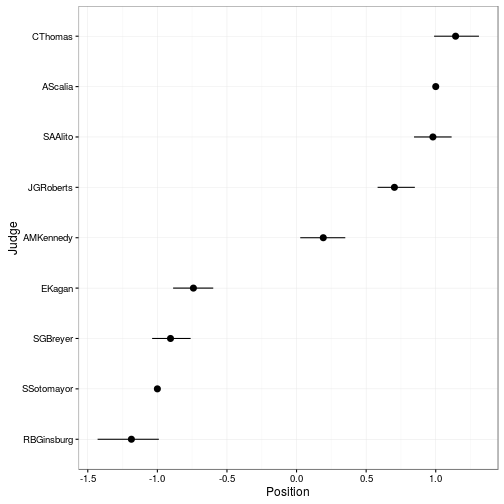
\includegraphics{figure/plotoutcomes-1.png}
\caption{Ideal points}
\end{figure}

\subsection{How good is the model?}\label{how-good-is-the-model}

\begin{itemize}
\tightlist
\item
  Has the model converged?
\item
  Does it make sense?

  \begin{itemize}
  \tightlist
  \item
    Do the judges line up in accordance with your priors?
  \item
    Is there a correlation between judge position and appointing party
    position?
  \item
    Do cases with large positive \(b\) result in ``conservative''
    outcomes?
  \end{itemize}
\item
  Does it fit the data well?

  \begin{itemize}
  \tightlist
  \item
    How many votes does it correctly predict?
  \item
    How does this compare to the null model (everyone votes with the
    majority with probability \(p\))
  \end{itemize}
\end{itemize}

\subsection{Extensions}\label{extensions}

\begin{itemize}
\tightlist
\item
  What if judges made decisions in two dimensions?

  \begin{itemize}
  \tightlist
  \item
    Possible, but tricky
  \item
    Data often not informative enough
  \item
    ``Informative voting'' (of the kind we see in legislatures) often
    one-dimensional
  \end{itemize}
\item
  What if we had extra information about judges (cases)?

  \begin{itemize}
  \tightlist
  \item
    Very possible: see \texttt{MCMirtHier1d}
  \end{itemize}
\end{itemize}

\subsection{Conclusions}\label{conclusions}

\begin{itemize}
\tightlist
\item
  Ideal point analysis is a form of description or data summary
\item
  It has a theory embedded within it
\item
  There are extensions which look at the cost of dissenting, or legal
  dimensions
\item
  \ldots{} but these are phenomenally complex:

  \begin{itemize}
  \tightlist
  \item
    Iaryczower, M., \& Shum, M. (2012). The value of information in the
    court: Get it right, keep it tight. \emph{The American Economic
    Review}, 102(1), 202-237.
  \item
    Weinshall Margel, K., Sommer, U, and Ritov, Y., (2016) Decision
    Making in High Courts: The Dynamic Comparative Attitudinal Measure.
    \emph{Working paper}.
  \end{itemize}
\end{itemize}

\hypertarget{refs}{}

\end{document}
